\documentclass[../thesis.tex]{subfiles}

\begin{document}

\chapter{Methodology}
\label{chap:method}

\noindent In this chapter we present the methodology and research structure used in this thesis. Some pre-processing of data including imputation and dimensional reduction will also be explained and presented. The implementation of the ML algorithms that produce the results presented in chapter (\ref{chap:exp}).

\section{Overview}

\noindent As stated in the chapter (\ref{chap:intro}), the aim of the thesis is split into two parts. The first part being that of seeing how well various clustering methods perform in producing phenotypically distinct clinical patient groups with HFpEF and HFmrEF? We frame the SL problem in the setting of unsupervised learning and accordingly use the following clustering methods: hierarchical clustering, k-Means and expectation-maximization to evaluate which produce the most clinically useful patient groups. The use of these clustering methods are common in the literature (see section \ref{subsec:unsupervisedlearn}) and serves as the main motivation for including them in our analysis. The second part of the problem statement looks at evaluating the accuracy of various classification algorithms in predicting the mortality and re-admission of patients with HFpEF and HFmrEF? In accordance with the literature as presented in section (\ref{sec:predclincout}), we reduce the SL problem of predicting the mortality and re-admission into a two class classification problem where both classes of outcomes are whether or not mortality/re-admission occurred. The classification methods that we will be evaluating are: k-nearest neighbours (k-NN), support vector machines (SVM), random forest and least absolute shrinkage and selection operator (LASSO) algorithms. All the algorithms are much used in the literature. The motivation behind the use of the chosen algorithms has always been to confirm with the practices done in the literature. We do however need to emphasize that many algorithms exists that can be used to further broaden the analysis done in this thesis. This is something we have not done due to limitations.


\begin{figure}

\centering
\small






\tikzset{every picture/.style={line width=0.75pt}} %set default line width to 0.75pt        

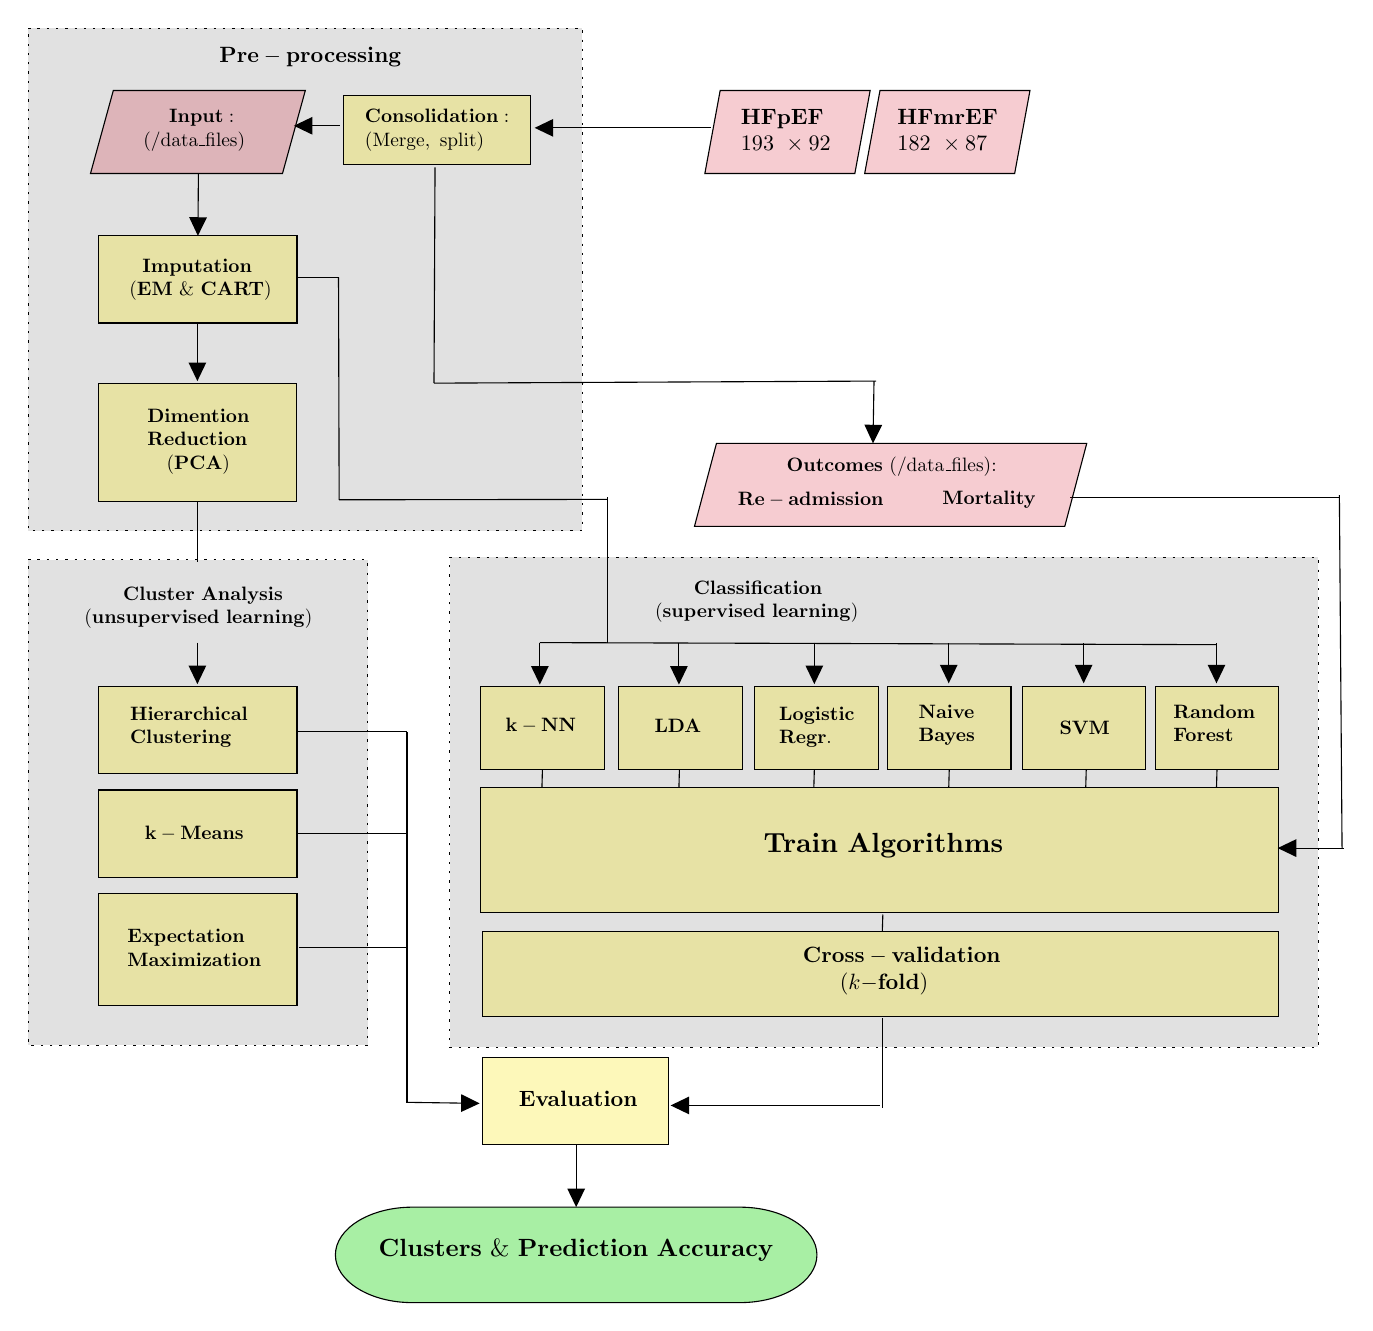
\begin{tikzpicture}[x=0.75pt,y=0.75pt,yscale=-1,xscale=1]
%uncomment if require: \path (0,646); %set diagram left start at 0, and has height of 646

%Shape: Rectangle [id:dp17767432122865645] 
\draw  [fill={rgb, 255:red, 155; green, 155; blue, 155 }  ,fill opacity=0.3 ][dash pattern={on 0.84pt off 2.51pt}] (2,5) -- (269,5) -- (269,247) -- (2,247) -- cycle ;
%Shape: Rectangle [id:dp17276791081063103] 
\draw  [fill={rgb, 255:red, 155; green, 155; blue, 155 }  ,fill opacity=0.3 ][dash pattern={on 0.84pt off 2.51pt}] (205,260) -- (623.5,260) -- (623.5,496) -- (205,496) -- cycle ;
%Shape: Rectangle [id:dp137712763597037] 
\draw  [fill={rgb, 255:red, 155; green, 155; blue, 155 }  ,fill opacity=0.3 ][dash pattern={on 0.84pt off 2.51pt}] (2,261) -- (165.5,261) -- (165.5,495) -- (2,495) -- cycle ;
%Straight Lines [id:da9350378875346577] 
\draw    (84,75) -- (83.77,103) ;
\draw [shift={(83.75,105)}, rotate = 270.48] [fill={rgb, 255:red, 0; green, 0; blue, 0 }  ][line width=0.75]  [draw opacity=0] (8.93,-4.29) -- (0,0) -- (8.93,4.29) -- cycle    ;

%Straight Lines [id:da9986924600189169] 
\draw    (83.5,147) -- (83.5,173) ;
\draw [shift={(83.5,175)}, rotate = 270] [fill={rgb, 255:red, 0; green, 0; blue, 0 }  ][line width=0.75]  [draw opacity=0] (8.93,-4.29) -- (0,0) -- (8.93,4.29) -- cycle    ;

%Straight Lines [id:da9104422198905568] 
\draw    (184.5,344) -- (184.5,523) ;


%Straight Lines [id:da17863107757037655] 
\draw    (184.5,522.5) -- (217.5,522.97) ;
\draw [shift={(219.5,523)}, rotate = 180.82] [fill={rgb, 255:red, 0; green, 0; blue, 0 }  ][line width=0.75]  [draw opacity=0] (8.93,-4.29) -- (0,0) -- (8.93,4.29) -- cycle    ;

%Straight Lines [id:da4423537570819638] 
\draw    (248.5,301) -- (248.5,319.22) ;
\draw [shift={(248.5,321.22)}, rotate = 270] [fill={rgb, 255:red, 0; green, 0; blue, 0 }  ][line width=0.75]  [draw opacity=0] (8.93,-4.29) -- (0,0) -- (8.93,4.29) -- cycle    ;

%Straight Lines [id:da14828368689404448] 
\draw    (315.5,301) -- (315.5,319.22) ;
\draw [shift={(315.5,321.22)}, rotate = 270] [fill={rgb, 255:red, 0; green, 0; blue, 0 }  ][line width=0.75]  [draw opacity=0] (8.93,-4.29) -- (0,0) -- (8.93,4.29) -- cycle    ;

%Straight Lines [id:da2745541849199835] 
\draw    (380.75,301) -- (380.75,319) ;
\draw [shift={(380.75,321)}, rotate = 270] [fill={rgb, 255:red, 0; green, 0; blue, 0 }  ][line width=0.75]  [draw opacity=0] (8.93,-4.29) -- (0,0) -- (8.93,4.29) -- cycle    ;

%Straight Lines [id:da10622223865111557] 
\draw    (445.5,301.39) -- (445.5,318.61) ;
\draw [shift={(445.5,320.61)}, rotate = 270] [fill={rgb, 255:red, 0; green, 0; blue, 0 }  ][line width=0.75]  [draw opacity=0] (8.93,-4.29) -- (0,0) -- (8.93,4.29) -- cycle    ;

%Straight Lines [id:da12728372488873485] 
\draw    (248.5,301) -- (574.5,302) ;


%Straight Lines [id:da04201945911359806] 
\draw    (413.5,482) -- (413.5,525) ;


%Straight Lines [id:da8309940078541183] 
\draw    (313.5,524) -- (412.5,524) ;

\draw [shift={(311.5,524)}, rotate = 0] [fill={rgb, 255:red, 0; green, 0; blue, 0 }  ][line width=0.75]  [draw opacity=0] (8.93,-4.29) -- (0,0) -- (8.93,4.29) -- cycle    ;
%Shape: Rectangle [id:dp805733141303524] 
\draw  [fill={rgb, 255:red, 248; green, 231; blue, 28 }  ,fill opacity=0.3 ] (220,371) -- (604.5,371) -- (604.5,431) -- (220,431) -- cycle ;
%Straight Lines [id:da5772744105119383] 
\draw    (281,231) -- (281,301) ;


%Straight Lines [id:da5307166780329797] 
\draw    (504,231) -- (634,231) ;


%Straight Lines [id:da8350224251535634] 
\draw    (633.71,230) -- (635,400) ;


%Shape: Rectangle [id:dp7689144799085996] 
\draw  [fill={rgb, 255:red, 248; green, 231; blue, 28 }  ,fill opacity=0.3 ] (36,105) -- (131.5,105) -- (131.5,147) -- (36,147) -- cycle ;
%Shape: Rectangle [id:dp8360402522569712] 
\draw  [fill={rgb, 255:red, 248; green, 231; blue, 28 }  ,fill opacity=0.3 ] (35.75,176) -- (131.25,176) -- (131.25,233) -- (35.75,233) -- cycle ;
%Shape: Rectangle [id:dp8436521642341313] 
\draw  [fill={rgb, 255:red, 248; green, 231; blue, 28 }  ,fill opacity=0.3 ] (36,322) -- (131.5,322) -- (131.5,364) -- (36,364) -- cycle ;
%Shape: Rectangle [id:dp8779924325569846] 
\draw  [fill={rgb, 255:red, 248; green, 231; blue, 28 }  ,fill opacity=0.3 ] (36,372) -- (131.5,372) -- (131.5,414) -- (36,414) -- cycle ;
%Shape: Rectangle [id:dp8944427225779763] 
\draw  [fill={rgb, 255:red, 248; green, 231; blue, 28 }  ,fill opacity=0.3 ] (36,422) -- (131.5,422) -- (131.5,476) -- (36,476) -- cycle ;
%Straight Lines [id:da12044404667160191] 
\draw    (131.5,344) -- (184.5,344) ;


%Straight Lines [id:da6084938483975053] 
\draw    (131.5,393) -- (184.5,393) ;


%Straight Lines [id:da16731103541967607] 
\draw    (132.5,448) -- (184.5,448) ;


%Straight Lines [id:da9753125405011336] 
\draw    (151.8,232.2) -- (281,232) ;


%Straight Lines [id:da8528567916678871] 
\draw    (151.5,125) -- (151.8,232.2) ;


%Straight Lines [id:da9889731806347037] 
\draw    (131.5,125) -- (151.5,125) ;


%Shape: Rectangle [id:dp8708975358842101] 
\draw  [fill={rgb, 255:red, 248; green, 231; blue, 28 }  ,fill opacity=0.3 ] (220,322) -- (279.5,322) -- (279.5,362) -- (220,362) -- cycle ;
%Shape: Rectangle [id:dp2832466894461272] 
\draw  [fill={rgb, 255:red, 248; green, 231; blue, 28 }  ,fill opacity=0.3 ] (286.5,322) -- (346,322) -- (346,362) -- (286.5,362) -- cycle ;
%Shape: Rectangle [id:dp14049594498977225] 
\draw  [fill={rgb, 255:red, 248; green, 231; blue, 28 }  ,fill opacity=0.3 ] (352,322) -- (411.5,322) -- (411.5,362) -- (352,362) -- cycle ;
%Shape: Rectangle [id:dp4503091833898072] 
\draw  [fill={rgb, 255:red, 248; green, 231; blue, 28 }  ,fill opacity=0.3 ] (416,322) -- (475.5,322) -- (475.5,362) -- (416,362) -- cycle ;
%Straight Lines [id:da37279512049375874] 
\draw    (249.5,371) -- (249.75,362) ;


%Straight Lines [id:da7877038245504153] 
\draw    (315.5,371) -- (315.75,362) ;


%Straight Lines [id:da47196717706905766] 
\draw    (380.5,371) -- (380.75,362) ;


%Straight Lines [id:da6265135418883228] 
\draw    (445.5,371) -- (445.75,362) ;


%Shape: Rectangle [id:dp23123927252195697] 
\draw  [fill={rgb, 255:red, 248; green, 231; blue, 28 }  ,fill opacity=0.3 ] (221,440) -- (604.5,440) -- (604.5,481) -- (221,481) -- cycle ;
%Straight Lines [id:da6647772541294572] 
\draw    (83.5,233) -- (83.5,262) ;


%Straight Lines [id:da7585523119166355] 
\draw    (413.5,440) -- (413.75,432) ;


%Straight Lines [id:da49016539083231736] 
\draw    (266,543) -- (266,571) ;
\draw [shift={(266,573)}, rotate = 270] [fill={rgb, 255:red, 0; green, 0; blue, 0 }  ][line width=0.75]  [draw opacity=0] (8.93,-4.29) -- (0,0) -- (8.93,4.29) -- cycle    ;

%Shape: Parallelogram [id:dp518581715076881] 
\draw  [fill={rgb, 255:red, 208; green, 2; blue, 27 }  ,fill opacity=0.2 ] (335.38,35) -- (407.64,35) -- (400.26,75) -- (328,75) -- cycle ;
%Straight Lines [id:da992949141941001] 
\draw    (83.5,301) -- (83.5,319) ;
\draw [shift={(83.5,321)}, rotate = 270] [fill={rgb, 255:red, 0; green, 0; blue, 0 }  ][line width=0.75]  [draw opacity=0] (8.93,-4.29) -- (0,0) -- (8.93,4.29) -- cycle    ;

%Straight Lines [id:da6160084227975695] 
\draw    (197.5,176) -- (410.5,175) ;


%Straight Lines [id:da3499925619434392] 
\draw    (409.5,175) -- (409.03,203) ;
\draw [shift={(409,205)}, rotate = 270.95] [fill={rgb, 255:red, 0; green, 0; blue, 0 }  ][line width=0.75]  [draw opacity=0] (8.93,-4.29) -- (0,0) -- (8.93,4.29) -- cycle    ;

%Straight Lines [id:da2578176252932385] 
\draw    (197.5,176) -- (198,72) ;


%Straight Lines [id:da924957907848829] 
\draw    (132,52) -- (152,52) ;

\draw [shift={(130,52)}, rotate = 0] [fill={rgb, 255:red, 0; green, 0; blue, 0 }  ][line width=0.75]  [draw opacity=0] (8.93,-4.29) -- (0,0) -- (8.93,4.29) -- cycle    ;
%Straight Lines [id:da09848220518746698] 
\draw    (248,53) -- (331,53) ;

\draw [shift={(246,53)}, rotate = 0] [fill={rgb, 255:red, 0; green, 0; blue, 0 }  ][line width=0.75]  [draw opacity=0] (8.93,-4.29) -- (0,0) -- (8.93,4.29) -- cycle    ;
%Shape: Parallelogram [id:dp8152627621795523] 
\draw  [fill={rgb, 255:red, 208; green, 2; blue, 27 }  ,fill opacity=0.2 ] (43,35) -- (135.5,35) -- (124.5,75) -- (32,75) -- cycle ;
%Shape: Parallelogram [id:dp9253495901859852] 
\draw  [fill={rgb, 255:red, 208; green, 2; blue, 27 }  ,fill opacity=0.2 ] (333.6,205) -- (512,205) -- (501.4,245) -- (323,245) -- cycle ;
%Shape: Parallelogram [id:dp42719482691252253] 
\draw  [fill={rgb, 255:red, 208; green, 2; blue, 27 }  ,fill opacity=0.2 ] (412.38,35) -- (484.64,35) -- (477.26,75) -- (405,75) -- cycle ;
%Flowchart: Terminator [id:dp16568399978235138] 
\draw  [fill={rgb, 255:red, 139; green, 233; blue, 134 }  ,fill opacity=0.75 ] (187.12,573) -- (344.88,573) .. controls (365.38,573) and (382,583.3) .. (382,596) .. controls (382,608.7) and (365.38,619) .. (344.88,619) -- (187.12,619) .. controls (166.62,619) and (150,608.7) .. (150,596) .. controls (150,583.3) and (166.62,573) .. (187.12,573) -- cycle ;
%Shape: Rectangle [id:dp14038294286941833] 
\draw  [fill={rgb, 255:red, 248; green, 231; blue, 28 }  ,fill opacity=0.3 ] (481,322) -- (540.5,322) -- (540.5,362) -- (481,362) -- cycle ;
%Shape: Rectangle [id:dp6127776736638881] 
\draw  [fill={rgb, 255:red, 248; green, 231; blue, 28 }  ,fill opacity=0.3 ] (545,322) -- (604.5,322) -- (604.5,362) -- (545,362) -- cycle ;
%Straight Lines [id:da7980328233946519] 
\draw    (510.5,301.39) -- (510.5,318.61) ;
\draw [shift={(510.5,320.61)}, rotate = 270] [fill={rgb, 255:red, 0; green, 0; blue, 0 }  ][line width=0.75]  [draw opacity=0] (8.93,-4.29) -- (0,0) -- (8.93,4.29) -- cycle    ;

%Straight Lines [id:da9962982021314886] 
\draw    (574.5,301.39) -- (574.5,318.61) ;
\draw [shift={(574.5,320.61)}, rotate = 270] [fill={rgb, 255:red, 0; green, 0; blue, 0 }  ][line width=0.75]  [draw opacity=0] (8.93,-4.29) -- (0,0) -- (8.93,4.29) -- cycle    ;

%Straight Lines [id:da5853970926877519] 
\draw    (606,400) -- (636,400) ;

\draw [shift={(604,400)}, rotate = 0] [fill={rgb, 255:red, 0; green, 0; blue, 0 }  ][line width=0.75]  [draw opacity=0] (8.93,-4.29) -- (0,0) -- (8.93,4.29) -- cycle    ;
%Shape: Rectangle [id:dp4763571703387559] 
\draw  [fill={rgb, 255:red, 248; green, 231; blue, 28 }  ,fill opacity=0.3 ] (221,501) -- (310.5,501) -- (310.5,543) -- (221,543) -- cycle ;
%Straight Lines [id:da7427067516231873] 
\draw    (511.5,371) -- (511.75,362) ;


%Straight Lines [id:da7011387804104916] 
\draw    (574.5,371) -- (574.75,362) ;



% Text Node
\draw (82,54) node [scale=0.7]  {$ \begin{array}{l}
\ \ \ \ \mathbf{Input:}\\
( /\mathrm{data\_files})
\end{array}$};
% Text Node
\draw (85,126) node [scale=0.7]  {$ \begin{array}{l}
\ \ \mathbf{Imputation}\\
\mathbf{( EM\ \&\ CART)}
\end{array}$};
% Text Node
\draw (84,204) node [scale=0.7]  {$ \begin{array}{l}
\mathbf{Dimention}\\
\mathbf{Reduction}\\
\ \ \ \mathbf{( PCA)}
\end{array}$};
% Text Node
\draw (81,342) node [scale=0.7]  {$ \begin{array}{l}
\mathbf{Hierarchical\ }\\
\mathbf{Clustering}
\end{array}$};
% Text Node
\draw (82,393) node [scale=0.7]  {$\mathbf{k-Means}$};
% Text Node
\draw (82,449) node [scale=0.7]  {$ \begin{array}{l}
\mathbf{Expectation}\\
\mathbf{Maximization}
\end{array}$};
% Text Node
\draw (84,284) node [scale=0.7]  {$ \begin{array}{l}
\ \ \ \ \ \ \mathbf{Cluster\ Analysis}\\
\mathbf{( unsupervised\ learning)}
\end{array}$};
% Text Node
\draw (249,341) node [scale=0.7]  {$\mathbf{k-NN}$};
% Text Node
\draw (315,341) node [scale=0.7]  {$\mathbf{LDA}$};
% Text Node
\draw (382,342) node [scale=0.7]  {$ \begin{array}{l}
\mathbf{Logistic}\\
\mathbf{Regr} .
\end{array}$};
% Text Node
\draw (446,341) node [scale=0.7]  {$ \begin{array}{l}
\mathbf{Naive\ }\\
\mathbf{Bayes}
\end{array}$};
% Text Node
\draw (414,459) node [scale=0.8]  {$ \begin{array}{l}
\ \ \ \ \ \mathbf{Cross-validation}\\
\ \ \ \ \ \ \ \ \ \ \mathbf{(} k\mathbf{-fold)}
\end{array}$};
% Text Node
\draw (353,281) node [scale=0.7]  {$ \begin{array}{l}
\ \ \ \ \ \ \mathbf{Classification}\\
\mathbf{( supervised\ learning)}
\end{array}$};
% Text Node
\draw (414,399) node   {$\mathbf{Train\ Algorithms}$};
% Text Node
\draw (266,594) node [scale=0.9]  {$\mathbf{Clusters\ \&\ Prediction\ Accuracy}$};
% Text Node
\draw (379,232) node [scale=0.7]  {$\mathbf{Re-admission}$};
% Text Node
\draw (465,232) node [scale=0.7]  {$\mathbf{Mortality}$};
% Text Node
\draw (418,216) node [scale=0.7]  {$\mathbf{Outcomes\ (} /\mathrm{data\_files})\mathbf{:}$};
% Text Node
\draw (445,55) node [scale=0.8]  {$ \begin{array}{l}
\mathbf{HFmrEF}\\
182\ \times 87
\end{array}$};
% Text Node
\draw (367,55) node [scale=0.8]  {$ \begin{array}{l}
\mathbf{HFpEF}\\
193\ \times 92
\end{array}$};
% Text Node
\draw  [fill={rgb, 255:red, 248; green, 231; blue, 28 }  ,fill opacity=0.3 ]  (154,37.5) -- (244,37.5) -- (244,70.5) -- (154,70.5) -- cycle  ;
\draw (199,54) node [scale=0.7]  {$ \begin{array}{l}
\mathbf{Consolidation} :\\
(\mathrm{Merge,\ split})
\end{array}$};
% Text Node
\draw (138,19) node [scale=0.8]  {$\mathbf{Pre-processing}$};
% Text Node
\draw (511,342) node [scale=0.7]  {$\mathbf{SVM}$};
% Text Node
\draw (575,341) node [scale=0.7]  {$ \begin{array}{l}
\mathbf{Random\ }\\
\mathbf{Forest}
\end{array}$};
% Text Node
\draw (267,521) node [scale=0.8]  {$\mathbf{Evaluation}$};

\end{tikzpicture}

\caption[Machine learning procedure adopted in the thesis]{\textit{Machine learning procedure adopted in the thesis}}
\label{fig:ML_proc_thesis}
\normalsize
\end{figure}

\indent The machine learning procedure adopted in this thesis is illustrated in figure (\ref{fig:ML_proc_thesis}). The structure starts by pre-processing the data. This pre-processing step consists of three sub processes: consolidation, imputation and dimension reduction. The consolidation process merges the HFpEF and HFmrEF dataset into one dataset with the same types of variables. In addition to having one dataset with all the observations, the process also leaves the data separate (but with equal variables) so that an analysis on each separate dataset can be done. Furthermore, the clinical outcomes of the patients in the dataset are extracted by this process and stored for later use in the classification part of thesis. The imputation process does imputation of missing data to ensure that the data is balanced and the dimensional reduction process addresses eventual problems with higher dimensional multi-correlated variables. The pre-processing steps are explained in further detail later in this chapter (see section \ref{sec:data}). After the pre-processing is done the structure continues by first addressing the cluster analysis. Being that the dimension reduction is relevant for both the cluster analysis and classification. We use the components derived from the dimension reduction process as input into both the clustering and classification algorithms evaluated. The cluster analysis runs the produced components through the three cluster algorithms (hierarchical clustering, k-Means and expectation maximization). After the procedure is done, three sets of clusters are produced and the next step is to evaluate the clusters to assess their medical usefulness. The supervised classification track on the other hand is structured in a somewhat different way. First the procedure starts by running the chosen components from the dimension reduction through the four classification algorithms (k-NN, SVM, RF and LASSO) and the data is trained and validated to produce approximately unbiased estimates of the test errors/accuracy. After the data is run thought the classification process and the accuracy are produced, the algorithms are ranked and evaluated accordingly. The outputs of the whole ML procedure are i) clinical clusters that \textit{may} have distinct phenotypical properties and ii) the accuracy of the various classification algorithms in predicting re-admission and mortality in the data sets. All the processes mentioned in the ML procedure in figure (\ref{fig:ML_proc_thesis}) are developed using the \texttt{R} statistical programming language (version 3.4.4 - \textit{Someone to Lean On}) \citep{Rsoftware2018} with RStudio as the integrated development environment (IDE), version 1.1.423 \citep{RStudio2018}. We use a number of external libraries and self-made algorithms in order to make the process more efficient. Data description with variable explanations, descriptive statistics and some relevant plot can be fount in appendix (\ref{chap:data_desc}). The source code used to produce all the results in this thesis can be found in appendix (\ref{chap:souce_code}). As we now have given an overview of the ML procedure used in this thesis we move on to presenting the data.

\section{Data}
\label{sec:data}

\noindent The data used is comprised of two data sets (\texttt{data\_use\_HFpEF.mat}, dim: $193 \times 92$ and \texttt{data\_use\_HFmrEF.mat}, dim: $182 \times 87$). Being that both datasets had different types of clinical variables, we consolidated the data into three dataset with the same number and types of variables: the full sample (\texttt{HFfullDataSet.Rdat}, dim: $374 \times 55$), the HFpEF sample (\texttt{HFpEFdataSet .Rdat}, dim: $193 \times 92$) and the HFmrEF sample (\texttt{HFmrEFdataSet.Rdat}, dim: $182 \times 87$).\\
\indent The data was collected by the medical staff at a tertiary hospital in the United Kingdom. At this particular hospital NT-proBNP led heart failure service were run on all patients with suspected heart failure. All patients with suspected HF based on an assessment of the HF probability and raised NT-proBNP/BNP levels (see figure \ref{fig:esc_algo_hf}) were included and forwarded for an echocardiography. An expert HF physician reviewed all the patients after the echocardiography was performed. The patients were diagnosed with HF according to the 2016 ESC guidelines \citep{ponikowski2016}. Accordingly, signs and symptoms of HF, raised NP values, echocardiographic results including left ventricular ejection fraction (LVEF) and evidence of structural or functional heart abnormalities were the primary basis for the assessment done by the hospitals cardiac physicians. After the diagnosis patients were categorized based on LVEF following the ESC guidelines, i.e. patients with LVEF $>$ 50\% were classified as HFpEF and those with $40 \leq$ LVEF $< 50$ as HFmrEF. The patients with LVEF $<$ 40\%, greater than moderate valvular heart disease and prior cardiac transplantation were excluded. The data was collected over a one year period from October 10th, 2014 to October 9th, 2015. In total 375 patients were analyzed over this one year period with data from 126 clinical features being recorded. The outcomes were evaluated through the hospitals databases and mortality was confirmed with the Office for National Statistics. All the data was collected as part of the hospitals approved Clinical Audit. As mentioned



\begin{footnotesize}
\begin{tabularx}{\textwidth}{LLLLLLLLLLL}
\caption{Clinical outcome classes}\label{tab:outcomes_class}\\
\toprule
\multicolumn{10}{c}{PANEL I: Full Sample (\texttt{HFfullDataSet.Rdat})}\\
\midrule
\multicolumn{2}{l}{\textbf{Group}} & \multicolumn{2}{l}{Dead?} & \multicolumn{2}{l}{Readm?} & \multicolumn{2}{l}{$n$} & \multicolumn{2}{l}{\% Tot}\\ 
\midrule
\multicolumn{2}{l}{R} &    \multicolumn{2}{l}{no}  & \multicolumn{2}{l}{no} &  \multicolumn{2}{l}{186} & \multicolumn{2}{l}{0.496} \\ 
\multicolumn{2}{l}{U} &    \multicolumn{2}{l}{no}  & \multicolumn{2}{l}{yes} & \multicolumn{2}{l}{59} &  \multicolumn{2}{l}{0.157} \\ 
\multicolumn{2}{l}{X, R} & \multicolumn{2}{l}{yes} & \multicolumn{2}{l}{no} &  \multicolumn{2}{l}{29} &  \multicolumn{2}{l}{0.077} \\ 
\multicolumn{2}{l}{Y} &    \multicolumn{2}{l}{yes} & \multicolumn{2}{l}{no} &  \multicolumn{2}{l}{16} &  \multicolumn{2}{l}{0.043} \\ 
\multicolumn{2}{l}{IN} &   \multicolumn{2}{l}{yes} & \multicolumn{2}{l}{no} &  \multicolumn{2}{l}{15} &  \multicolumn{2}{l}{0.040}\\ 
\multicolumn{2}{l}{V} &    \multicolumn{2}{l}{no}  & \multicolumn{2}{l}{yes} & \multicolumn{2}{l}{15} &  \multicolumn{2}{l}{0.040}\\ 
\multicolumn{2}{l}{Y, U} & \multicolumn{2}{l}{yes} & \multicolumn{2}{l}{yes} & \multicolumn{2}{l}{13} &  \multicolumn{2}{l}{0.035} \\ 
\multicolumn{2}{l}{X, U} & \multicolumn{2}{l}{yes} & \multicolumn{2}{l}{yes} & \multicolumn{2}{l}{11} &  \multicolumn{2}{l}{0.029} \\ 
\multicolumn{2}{l}{Y, V} & \multicolumn{2}{l}{yes} & \multicolumn{2}{l}{yes} & \multicolumn{2}{l}{11} &  \multicolumn{2}{l}{0.029} \\ 
\multicolumn{2}{l}{X} &    \multicolumn{2}{l}{yes} & \multicolumn{2}{l}{no} &  \multicolumn{2}{l}{9 }&   \multicolumn{2}{l}{0.024} \\ 
\multicolumn{2}{l}{Z} &    \multicolumn{2}{l}{yes} & \multicolumn{2}{l}{no} &  \multicolumn{2}{l}{7 }&   \multicolumn{2}{l}{0.019} \\ 
\multicolumn{2}{l}{X, V} & \multicolumn{2}{l}{yes} & \multicolumn{2}{l}{yes} & \multicolumn{2}{l}{3 }&   \multicolumn{2}{l}{0.008} \\ 
\multicolumn{2}{l}{Z, V} & \multicolumn{2}{l}{yes} & \multicolumn{2}{l}{yes} & \multicolumn{2}{l}{1 }&   \multicolumn{2}{l}{0.003} \\ 
\midrule
\multicolumn{10}{c}{PANEL II: Outcome Classes by Clinical Syndrome}\\
\midrule
\multicolumn{5}{c}{HFpEF (\texttt{HFpEFdataSet.Rdat})} & \multicolumn{5}{c}{HFmrEF (\texttt{HFmrEFdataSet.Rdat})}\\
\midrule
\textbf{Group} & Dead? & Readm? & $n$ & \% Tot & \textbf{Group} & Dead? & Readm? & $n$ & \% Tot \\ 
\midrule
R & no & no & 85 & 0.440 & R & no & no & 101 & 0.555 \\ 
U & no & yes & 40 & 0.207 & U & no & yes & 19 & 0.104 \\ 
X, R & yes & no & 29 & 0.150 & Y & yes & no & 15 & 0.082 \\ 
V & no & yes & 10 & 0.052 & IN & yes & no & 8 & 0.044 \\ 
IN & yes & no & 7 & 0.036 & X & yes & no & 8 & 0.044 \\ 
Y, U & yes & yes & 7 & 0.036 & Z & yes & no & 7 & 0.038 \\ 
Y, V & yes & yes & 7 & 0.036 & Y, U & yes & yes & 6 & 0.033 \\ 
X, U & yes & yes & 6 & 0.031 & V & no & yes & 5 & 0.027 \\ 
X & yes & no & 1 & 0.005 & X, U & yes & yes & 5 & 0.027 \\ 
Y & yes & no & 1 & 0.005 & Y, V & yes & yes & 4 & 0.022 \\ 
&  &  &  &  & X, V & yes & yes & 3 & 0.016 \\ 
&  &  &  &  & Z, V & yes & yes & 1 & 0.005 \\
\midrule
\end{tabularx}
\end{footnotesize}

\newpage

\noindent in the previous section, we reduced the SL problem in the supervised learning part of the ML procedure to that of a two class classification problem. The way in which this was done was with respect to the various \texttt{patient\_groups} in the data. The patients were grouped based on various \noindent outcomes. In total six outcome categories were  defined in the data sets. The outcome categories are as follows: \texttt{IN} - inhospital death, \texttt{Z} \noindent dead within 30 days, \texttt{Y} - dead within 1 year, \texttt{X} - dead by Fluorouracil (medication), \texttt{V} - cardiac readmission within 30 days, \texttt{U} - readmission and \texttt{R} - the rest. The various combinations of the outcome classes found in the data sets and the way in which they were classified are listed in table (\ref{tab:outcomes_class}).\\
\indent From this table we can see that approximately 36.8\% of all the patients in the HFpEF data set were readmitted in some form, i.e either within 30 days or more. In the HFmrEF data set this number was somewhat smaller being approximately 23.4\%. In the full sample approximately 29.1\% of the patients were readmitted. The number also differed with respect to the whether the patients were confirmed deceased or not. In the HFpEF data set approximately 29.9\% of the patients were confirmed deceased and in the HFmrEF data set this number was 31.1\%. For the full sample this number is approximately 30.7\%. Further descriptive statistics on the data can be found in appendix (\ref{sec:desc_stat}). The source code for the two-class outcome classification shown in table (\ref{tab:outcomes_class}) can be found in appendix (\ref{sec:app_desc_stat}). As the data used in this thesis is cross-sectional, we need to emphasize that it is not perfect. Limitations to the data sets are many and one of the most primary of them is regarding missing data. 

\subsection{Missing Data}
\label{subsec:miss_data}

\noindent Missing values in data is a very important concept in data management and a highly prevalent problem in any data analysis. If one does not handle missing values properly this may lead to inaccurate or invalid inference being drawn from the data. Results where improper treatment of missing data is present may differ significantly from those where missing data is not present. In medical research it is not uncommon for patient data to be missing. Missing data from patients clinical variables are typically defined as the values that are not directly observed \citep{ibrahim2012missing}. Data can be missing due to a number of reasons. In clinical research some reasons may include: poor communication with study subject, difficulties assessing the clinical outcomes, lack of consolidation from test, duration of trial etc. The latter is often a reason for missing data as longer trials tend to produce more risk of missing data. Especially considering that patients often run the risk of being dropped from the studies before completion \citep{myers2000handling}.



\begin{footnotesize}
\begin{tabularx}{\textwidth}{P{2.3cm}LLLLP{2.7cm}LLLL}
\caption{Summary of missing values}\label{tab:top_missing}\\
\toprule
\multicolumn{10}{c}{PANEL I: Full Sample (\texttt{HFfullDataSet.Rdat})}\\
\midrule
\multicolumn{2}{l}{\textbf{Variable (V)}}& \multicolumn{2}{l}{\#Na} & \multicolumn{2}{l}{\%$n$} & \multicolumn{2}{l}{\%Na} & \multicolumn{2}{l}{\%V} \\ 
\midrule
\multicolumn{2}{l}{grand.tot      } & \multicolumn{2}{l}{3081}  & \multicolumn{2}{l}{0.149} & \multicolumn{2}{l}{1.000} & \multicolumn{2}{l}{     } \\ 
\midrule
\multicolumn{2}{l}{irondef        } & \multicolumn{2}{l}{254 }  & \multicolumn{2}{l}{0.012} & \multicolumn{2}{l}{0.082} & \multicolumn{2}{l}{0.677} \\ 
\multicolumn{2}{l}{ferritin       } & \multicolumn{2}{l}{250 }  & \multicolumn{2}{l}{0.012} & \multicolumn{2}{l}{0.081} & \multicolumn{2}{l}{0.667} \\ 
\multicolumn{2}{l}{bmiadmission   } & \multicolumn{2}{l}{223 }  & \multicolumn{2}{l}{0.011} & \multicolumn{2}{l}{0.072} & \multicolumn{2}{l}{0.595} \\ 
\multicolumn{2}{l}{ironlevels     } & \multicolumn{2}{l}{210 }  & \multicolumn{2}{l}{0.010} & \multicolumn{2}{l}{0.068} & \multicolumn{2}{l}{0.560} \\ 
\multicolumn{2}{l}{tsat           } & \multicolumn{2}{l}{210 }  & \multicolumn{2}{l}{0.010} & \multicolumn{2}{l}{0.068} & \multicolumn{2}{l}{0.560} \\ 
\multicolumn{2}{l}{timetohfadm    } & \multicolumn{2}{l}{184 }  & \multicolumn{2}{l}{0.009} & \multicolumn{2}{l}{0.060} & \multicolumn{2}{l}{0.491} \\ 
\multicolumn{2}{l}{pasp           } & \multicolumn{2}{l}{181 }  & \multicolumn{2}{l}{0.009} & \multicolumn{2}{l}{0.059} & \multicolumn{2}{l}{0.483} \\ 
\multicolumn{2}{l}{admissionwgt   } & \multicolumn{2}{l}{164 }  & \multicolumn{2}{l}{0.008} & \multicolumn{2}{l}{0.053} & \multicolumn{2}{l}{0.437} \\ 
\multicolumn{2}{l}{ecgqrsduration } & \multicolumn{2}{l}{141 }  & \multicolumn{2}{l}{0.007} & \multicolumn{2}{l}{0.046} & \multicolumn{2}{l}{0.376} \\ 
\multicolumn{2}{l}{obesity        } & \multicolumn{2}{l}{137 }  & \multicolumn{2}{l}{0.007} & \multicolumn{2}{l}{0.044} & \multicolumn{2}{l}{0.365} \\ 
\midrule
\multicolumn{5}{c}{HFpEF (\texttt{HFpEFdataSet.Rdat})} & \multicolumn{5}{c}{HFmrEF (\texttt{HFmrEFdataSet.Rdat})}\\
\midrule
\textbf{Variable (V)}& \#Na & \%$n$ & \%Na & \%V & \textbf{Variable (V)} & \#Na & \%$n$ & \%Na & \%V \\ 
\midrule
grand.tot &         973 & 0.092 & 1 &  & grand.tot & 2108 & 0.211 & 1 &  \\ 
\midrule
irondef & 124 & 0.012 & 0.127 & 0.642 & bmiadmission & 178 & 0.018 & 0.084 & 0.978 \\ 
timetohfadm & 124 & 0.012 & 0.127 & 0.642 & admissionwgt & 131 & 0.013 & 0.062 & 0.720 \\ 
ferritin & 122 & 0.011 & 0.125 & 0.632 & irondef & 130 & 0.013 & 0.062 & 0.714 \\ 
tsat & 99 & 0.009 & 0.102 & 0.513 & obesity & 129 & 0.013 & 0.061 & 0.709 \\ 
ironlevels & 98 & 0.009 & 0.101 & 0.508 & ferritin & 128 & 0.013 & 0.061 & 0.703 \\ 
pasp & 71 & 0.007 & 0.073 & 0.368 & breathless & 127 & 0.013 & 0.060 & 0.698 \\ 
bmiadmission & 45 & 0.004 & 0.046 & 0.233 & ironlevels & 112 & 0.011 & 0.053 & 0.615 \\ 
ee & 41 & 0.004 & 0.042 & 0.212 & tsat & 111 & 0.011 & 0.053 & 0.610 \\ 
ecgqrsduration & 36 & 0.003 & 0.037 & 0.187 & pasp & 110 & 0.011 & 0.052 & 0.604 \\ 
ecgrate & 34 & 0.003 & 0.035 & 0.176 & ecgqrsduration & 105 & 0.010 & 0.050 & 0.577 \\
\midrule
\end{tabularx}
\end{footnotesize}

\indent In our data sets the problem with missing values is very much present. In the full data set, a total of 3081 observations are missing accounting for about 14.9\% of the total data set. The main non-indicator variables accounting for the highest amount of this number is the lack of registering ferritin levels (\texttt{ferritin}, 8.1\% of missing), BMI at admission (\texttt{bmiadmission}, 7.2\%), ironlevels (\texttt{ironlevels}, 6.8\%), transferrin saturation (\texttt{tsat}, 6.8\%), time of HF admission (\texttt{timetohfadm}, 6\%), pulmonary artery systolic pressure (\texttt{pasp}, 5.9\%), weight at admission (\texttt{admissionwgt}, 5.3\%) and ECQ QRS duration (4.6\%). We can also look at the missing values in both the sub datasets. In the HFpEF data set a total of 973 observations, i.e. approximately 9.2\% of the data set is missing. Of the non-indicator variables, the largest contributors can be attributed to the failure of registering time to HF admission (\texttt{timetohfadm}, 12.7\% of missing), ferritin levels (\texttt{ferritin}, 12.5\%), transferrin saturation (\texttt{tsat}, 10.2\%), iron levels (\texttt{ironlevels}, 10.1\%), pulmonary artery systolic pressure (\texttt{pasp}, 7.3\%), registering body-mass-index (BMI) at admission (\texttt{bmiadmission}, 4.6\%), E/e' ratio (\texttt{ee}, 4.2\%), ECQ QRS duration (\texttt{ecgqrsduration}, \texttt{3.7\%}) and ECG rate (\texttt{ecgrate}, 3.5\%). These variables contribute to approximately 68.8\% of the missing values in the HFpEF data. In the HFmrEF data set, the picture is very much different. In general we can say that this data set has a much larger presence of missing values. Even as the clinical variables used in both sets are the same. In total 2108 observations, i.e. approximately 21.1\% of the data is missing. The largest non-indicator contributors are: inability to record the body mass index (BMI) at admission (\texttt{bmiadmission}, 8.4\%), the weight of patients at admission (\texttt{admissionwgt}, 6.2\%), ferritin levels (\texttt{ferritin}, 6.1\%), iron levels (\texttt{ironlevels}, 5.3\%), transferrin saturation (\texttt{tsat}, 5.3\%), pulmonary artery systolic pressure (\texttt{pasp}, 5.2\%) and ECQ QRS duration (\texttt{ecgqrsduration}, \texttt{5\%}). These variables account for 41.1\% of the missing values in the HFmrEF data. An overview of the variables with the most missing values in each data set can be found in table (\ref{tab:top_missing}).

\subsection{Little's Test for MCAR}
\label{subsec:little}

\noindent The presence of missing values is something that needs to be addressed by any individual conducting data analysis. As missing values makes the data corrupted and may introduce statistical bias that may lead to invalid results and inferences. This is vital for us as many of the statistical methods used later in this thesis cannot be conducted in the presence of missing values. When talking about missing values one typically mentions three distinct types of missing values, see e.g. \cite{sterne2009multiple} and \cite{kaushal2014missing} for further explanation. These are as follows:

\newpage

\begin{enumerate}[label=(\roman*)]
    \item Missing completely at random (MCAR): This type assume that there is no systematic difference between the missing values and the observed values. Some example can be if blood pressure values are missing due to breakdown in automatic sphygmomanometer or if blood sugar values are missing due to non working glucometer.
    \item Missing at random (MAR): The second type of missing values assume that any difference between the missing values and the observed values can be explained by differences in the observed values. Again an example can be that missing blood pressure values or blood sugar values may be lower than the measured values but only because younger people may be more likely to have missing blood pressure and blood sugar as missing.
    \item Missing not at random (MNAR): The last and final type assumes that even after the observer data are taken into account, the systematic differences between the observed and missing values are still present. An example can be that people with high values of blood pressure or blood sugar may be less likely to go to appointment due to headache.  
\end{enumerate}

\noindent The last type of missing value can only be speculated and thus never determined, see e.g. \cite{rubin1976inference}, \cite{schafer2002missing} and \cite{moons2006using}. In our data, we assume that the missing data is at least missing at random (MAR). This is an assumption that many in the literature place on their data without an attempt at supplying some arguments to support such an assumption. To this we have carried out Little's MCAR test \citep{little1988test} on our data (separately on indicator and continuous variables). The test is structured with the following three steps : 
\begin{enumerate}[label=(\roman*)]
    \item First the test starts by using the expectation-maximization (EM) algorithm \citep{dempster1977maximum} to estimate the maximum likelihood of the population mean $\bm{\tilde{\mu}}_{obs, j}$ and variance-covariance matrix $\bm{\tilde{\Sigma}}_{obs,j}$. Here one enters the $Y:N\times p$ matrix of data into the EM algorithm.
    \item Next step is to create a set of matrices $S_j$ for $j = 1, \hdots, J$ where each matrix of the dataset consists of all cases that are identified with particular missing patterns (0 = not-missing and 1 = missing). Define $m_j$ to be the number of cases that belong to a given missing response pattern in $S_j$. From these $J-1$ cases, calculate the \textit{observed} vector of means $\bm{\hat{y}}_{obs, j}$ for each random response pattern. 
    \item The final step comprises of calculating the difference between the observed means in step 2 with the estimated EM-means from step 1 weighted by $m_j$ and the inverse variance-covariance matrix to obtain the the following test statistics:
    \begin{align}
        d^2 = \sum_{j=1}^J m_j \left(\bm{\hat{y}}_{obs, j} -  \bm{\tilde{\mu}}_{obs, j}\right)\bm{\tilde{\Sigma}}_{obs,j}^{-1}\left(\bm{\hat{y}}_{obs, j} -  \bm{\tilde{\mu}}_{obs, j}\right)^T
    \end{align}
\end{enumerate}

\noindent \cite{little1988test} showed that $d^2$ is asymptotically $\chi^2$-distributed with $f = \sum_{j=1}^J p_j - p$ degrees of freedom, where $p_j$ is the number of observed variables for cases in $S_j$. Thus with the use of $d^2$, a large-sample test of the MCAR assumption compares $d^2$ with a chi-squared distribution with $f$ df can be done, and rejecting the null hypothesis when $d^2$ is large. Following this procedure, we have carried out Little's MCAR test and the results are presented in table (\ref{tab:little_test}). The results were produces using the function \texttt{LittleMCAR()} in the \texttt{r} package \texttt{BaylorEdPsych} \citep{BaylorEdPsych}. We removed the variables that had more than 15\% missing values from the


\begin{footnotesize}
\begin{tabularx}{\textwidth}{Lrrrrr}
\caption{Little's MCAR test}\label{tab:little_test}\\
\toprule
& num col & missing.patterns & Chi.squared ($\chi^2$) & df & $p$-value\\
\midrule
\endfirsthead
\caption*{\textbf{Table \ref{tab:little_test}:} Little's MCAR test (\textit{continued})}\\
\toprule
& num col & missing.patterns & Chi.squared ($\chi^2$) & df & $p$-value\\
\midrule
\endhead
\multicolumn{6}{c}{Panel I: HFpEF}\\
\midrule
indicator & 43 & 37 & 692.8908 & 662 & 0.19645 \\ 
continuous\_1 & 16 & 58 & 534.3060 & 542 & 0.58493 \\ 
continuous\_2 & 16 & 83 & 720.2238 & 751 & 0.78464 \\ 
continuous\_3 & 17 & 49 & 330.3824 & 383 & 0.97567 \\
\midrule
\multicolumn{6}{c}{Panel II: HFmrEF}\\
\midrule
indicator.1 & 49 & 135 & 2331.4367 & 2276 & 0.20470 \\ 
continuous\_1.1 & 15 & 71 & 409.6785 & 440 & 0.84708 \\ 
continuous\_2.1 & 15 & 19 & 106.9243 & 105 & 0.42938 \\
\midrule
\end{tabularx}
\end{footnotesize} 

\noindent HFpEF dataset and 20\% from the HFmrEF dataset (see table \ref{tab:top_missing} for top 10 missing variables). Next, we split the variables into to two datasets, one for the continuous variables and one for the indicator variables. We also removed the variables that had near zero variance using the \texttt{nearZeroVar()} function in the \texttt{caret} package \citep{kuhncaret}. As remarked by \cite{BaylorEdPsych}, the \texttt{LittleMCAR()} function can be very time inefficient for datasets with more than 50 variables. This time inefficiency is why we split the datasets into the two subsets, i.e. continuous and indicator and thus conducted separate tests on both subsets. The test assumes that the data is MCAR, and this is accordingly the null-hypothesis. From table (\ref{tab:little_test}), we can see that all the $p$-values are insignificant at 5\% significance level. Suggesting that we cannot reject the null hypothesis of the missing data  
\noindent being MCAR. However, as argued by \cite{allison1999missing}, just because the data passes this test does not mean that the MCAR assumption is satisfied. The assumptions for MCAR are strong and a simple test such as the one suggested by \cite{little1988test}, does not in and of itself satisfy those assumptions. It merely lends evidence in its support and given the test results presented in table (\ref{tab:little_test}) we consider this assumption to be intact. When it comes to the question regarding missing values there exists many ways of dealing with this problem. Each of these ways have different disadvantages as well as advantages. One of the most used ways of dealing with missing values is through the use of imputation techniques. 

\subsection{Imputation}
\label{subsec:impu}

\noindent There exists a wide variety of methods that fall under the class of imputation. In general all methods that attempt to replace each missing value in a dataset with an estimate or a guess are typically classified as being an imputation method \citep{allison1999missing}. A very popular and conventional method of imputing missing values is through the use of mean imputation. This method implies swapping each missing value with the mean of the observed values in the given variable column. The method is very easy to use and maintains the sample size, but it has a problem with underestimating both the variance and standard deviation estimates. This implies that the estimates that the produced imputed values are unbiased see e.g. \cite{scheffer2002dealing}, \cite{enders2010applied} and \cite{eekhout2012brief}. Another class of imputation methods that have proven to handle missing values in a wide variety of cases is the maximum likelihood methods. The use of set method requires that the assumption of MCAR is intact and as such if this is done can produce estimates that have the desirable properties normally associated with maximum likelihood. These properties are consistency (estimates will be approximately unbiased in large samples), asymptotic efficiency (estimates are close to being fully efficient i.e., having minimal standard errors) and asymptotic normality (allows the use of normal approximation to calculate confidence intervals and $p$-values). Additionally, the use of maximum likelihood methods can produce standard errors that fully account for the fact that some data is missing \citep{allison1999missing}. Its exactly based on these qualities that we have chosen maximum likelihood based imputation as one of the strategies to address the problem with the missing values in our data set presented in subsection (\ref{subsec:miss_data}). We also showed that this is relevant as the assumption of MCAR is assumed intact, see subsection (\ref{subsec:little}).\\
\indent A maximum likelihood method typically starts out by expressing a likelihood function. This function expresses the probability of the data as a function of the unknown parameters. If we assume two discrete random variables: $\mathbf{X}$ and $\mathbf{Z}$ with a joint probability function defined by $p(x,z|\boldsymbol{\theta})$, where $\boldsymbol{\theta}$ is a vector of parameters. This joint probability function gives us the probability that $\mathbf{X} = x$ and $\mathbf{Z} = z$. If we assume that there are no missing values and that the observations are independent, i.e. $cov(\mathbf{X}, \mathbf{Z}) = 0$. Then the likelihood function is defined by:
\begin{align}
    L(\boldsymbol{\theta}) = \prod_{i=1}^n p(x_i, z_i | \boldsymbol{\theta})
    \label{eq:likelihood}
\end{align}
\noindent To find an estimate of the maximum likelihood, we need to find the value for $\boldsymbol{\theta}$ that maximizes the likelihood function (eq. \ref{eq:likelihood}). This can be done using the log-likelihood function ($\mathcal{L} (\boldsymbol{\theta}) = \log L(\boldsymbol{\theta})$) and should give us an estimate defined by:
\begin{align}
    {\displaystyle {\hat {\theta }}\in \left \{{\underset {\theta \in \Theta }{\operatorname {arg\,max} }}\ \sum_{i=1}^n\log p (x_i, z_i | \boldsymbol{\theta})\right \}}
\end{align}
\noindent If we assume that the data is MAR on $\boldsymbol{Z}$ for the first $r$ cases, and MAR on $\boldsymbol{X}$ for the next $s$ cases. Then we can split the likelihood function into parts that correspond to each missing value pattern and accordingly factor these parts. This in order to get a likelihood function that takes into account the missing data patterns. Then the likelihood function becomes:
\begin{align}
    L(\boldsymbol{\theta}) = \prod_{i=1}^r g(x_i | \boldsymbol{\theta})\prod_{i=r+1}^{r+s} h(z_i | \boldsymbol{\theta})\prod_{i=r+s+1}^n p(x_i, z_i | \boldsymbol{\theta}) 
\end{align}
\noindent where $g(x | \theta)$ and $h(z | \theta)$ are the marginal distributions of $\boldsymbol{X}$ and $\boldsymbol{Z}$, so that:
\begin{align}
    \prod_{i = 1}^r g(x_i | \boldsymbol{\theta}) \prod_{i = r + 1}^{r + s} h(z_i | \boldsymbol{\theta}) = \prod_{i=1}^{r+s} p(x_i, z_i | \boldsymbol{\theta})
\end{align}
\noindent For each missing data pattern, the likelihood is found by summing the joint distribution over all possible values of the variables with missing data. So the estimated maximum likelihood parameters in this particular example should be defined by:
\begin{align}
    {\displaystyle {\hat {\theta }}\in \left \{{\underset {\theta \in \Theta }{\operatorname {arg\,max} }}\ \left(\sum_{i=1}^{r+s}\log p(x_i, z_i | \boldsymbol{\theta}) + \sum_{i=r+s+1}^n\log p (x_i, z_i | \boldsymbol{\theta})\right)  \right\}}
\end{align}
\noindent Keep in mind that we assumed that the variables were discrete in the begin, and as such if the variables were continuous then the summations would be replaced by integrals as the following. The extension to multiple variables is also relatively straightforward \citep{allison1999missing}. In order to implement a maximum likelihood method on data that contains missing values its important to have a model for the joint distribution for all variables in the data set, and accordingly have a numerical method for maximizing the likelihood of this distribution. Determining this model can vary with the type of data that one is dealing with.\\
\indent In our data set, we have both continuous and indicator variables. When the data is continuous its common to assume a multivariate-normal model, i.e. that all the variables are independently identically normally distributed (iid) and can be expressed as a linear function of all other variables (or subsets). There is also an assumption that the errors are homoscedastic, i.e. constant and have a mean of 0. In the case of the indicator variables, its difficult to assume that these variables are normally distributed. However, according to \cite{schafer1997analysis}, \cite{schafer1998multiple} and \cite{allison1999missing} simulation evidence and practical experience have shown that maximum likelihood methods can do a god job in imputing missing values even if the variables in question are indicator variables. Still, we have adopted to use a different imputation methods for each of the types of data, i.e. we use a bootstrapped expectation-maximization (EM) imputation method for the variables that are continuous and a classification- and regression tree (CART) based imputation method for the indicator variables.\\
\indent As we mentioned one needs to have a numerical method for maximizing the likelihood of the joint probability distribution. One of the most common numerical methods for doing just this is the expectation-maximization (EM) algorithm \citep{dempster1977maximum}. We mentioned it slightly in subsection (\ref{subsec:little}), but it is an iterative algorithm that is used to maximize the likelihood function (eq. \ref{eq:likelihood}) of a number of missing data models. It is comprised of two steps, the expectation step (often called the $E$ step) and the maximization step (called the $M$ step). In the expectation step the expected values of the log-likelihood is taken over the variables with missing values using the current estimated parameters \citep{allison1999missing}. After this is done the maximization step involves maximizing the expected log-likelihood in order to get new estimates of the parameters. These two step are continued until convergence is achieved, i.e. until the estimated parameters of the joint probability distribution do not change from one iteration until the next. Most standard software packages using an EM implementation have as a principal output a set of maximum likelihood parameters related to the joint probability distribution. The imputed values are often included in addition, but are not recommended for further analysis. The reason for this is that these imputed values are not designed for that purpose and as such will produce biased estimates of many parameters if used in further analysis \citep{allison1999missing}.\\
\indent A way to get around this problem is by using multiple-imputation. \cite{honaker2011amelia}  introduced a bootstrapped EM algorithm that combines the nice properties of the EM algorithm, i.e. consistency, asymptotic efficiency etc. with the accuracy property of the bootstrap re-sampling method, see \cite{efron1992bootstrap} and \cite{james2013introduction}. \cite{honaker2011amelia} also argue that the EMB algorithm they developed is much faster and more reliable than alternative algorithms. In addition to making valid and much more accurate imputations for cross-sectional data. The algorithm is implemented in the \texttt{Amalie II} package in \texttt{r}. The assumptions of the algorithm are: If we assume that the data set can be expressed as a matrix $\boldsymbol{D}$ consisting of dimensions $(n\times k)$. Let the matrix $\boldsymbol{D}$ be comprised of two parts, i.e. $\boldsymbol{D^{mis}}$ the missing part and $\boldsymbol{D^{obs}}$ the observer part. The matrix $\boldsymbol{D}$ is assumed to follow a multivariate distribution with mean vector $\boldsymbol{\mu}$ and covariance matrix $\boldsymbol{\Sigma}$. This assumption can be stated as $\boldsymbol{D} \sim N\left(\boldsymbol{\mu},  \boldsymbol{\Sigma}\right)$. In addition to the multivariate normality assumption, the algorithm assumes that the data is MAR. The latter have we already shown to be intact, but the first assumption is somewhat difficult. As the data is by definition incomplete due to the missing data, we assume that this assumption intact. Typically one would test if this assumption is intact using a multivariate normality test similar to the ones mentioned by \cite{mardia1970measures}, \cite{henze1990class} or \cite{royston1982extension}. Most of these tests assume that the data is complete, and should the data be incomplete then its common to remove the missing observations and conduct the tests on the remaining data. The challenge for our part is that approximately 15\% of our data set is missing which may cast doubt on the loss of statistical power that these tests may have. As a result of this we have chosen to assume that the normality assumption is intact. The schematic approach of this algorithm and the way it used in this thesis is described in Figure (\ref{fig:BEM_algo}). The procedure starts by producing $n$ bootstrapped data sets for which the EM algorithm is run on each bootstrapped data sets. In the full data sample (\texttt{HFfullDataSet.Rdat}) we let the algorithm produce $n = 20$ bootstrapped data sets, whilst for the other data sets, i.e. \texttt{HFpEFdataSet.Rdat} and \texttt{HFmrEFdataSet.Rdat} we use $n = 100$. After the imputed data sets are produced they are collapsed by averaging all the imputed values produced by the EM algorithm. All the data from the incomplete data set that the procedure started with should be the same with the exception of the missing values, i.e. these have be replaced by the average of the imputed values.

\begin{figure}

\centering





\tikzset{every picture/.style={line width=0.75pt}} %set default line width to 0.75pt        

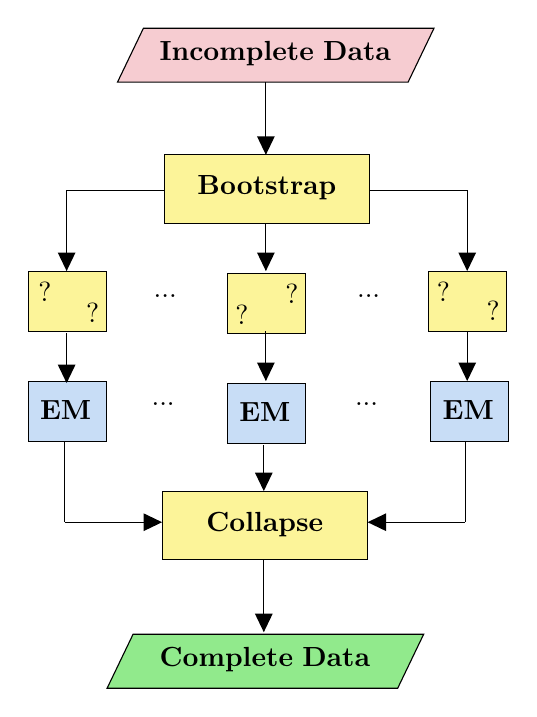
\begin{tikzpicture}[x=0.75pt,y=0.75pt,yscale=-1,xscale=1]
%uncomment if require: \path (0,652); %set diagram left start at 0, and has height of 652

\draw  [fill={rgb, 255:red, 208; green, 2; blue, 27 }  ,fill opacity=0.2 ] (244.5,3) -- (384.5,3) -- (372,29) -- (232,29) -- cycle ;
\draw    (303.5,29) -- (303.5,62) ;
\draw [shift={(303.5,64)}, rotate = 270] [fill={rgb, 255:red, 0; green, 0; blue, 0 }  ][line width=0.75]  [draw opacity=0] (8.93,-4.29) -- (0,0) -- (8.93,4.29) -- cycle    ;

\draw  [fill={rgb, 255:red, 248; green, 231; blue, 28 }  ,fill opacity=0.45 ] (254.5,64) -- (353.5,64) -- (353.5,97) -- (254.5,97) -- cycle ;
\draw    (207.5,81) -- (254.5,81) ;


\draw    (353.5,81) -- (400.5,81) ;


\draw    (207.5,81) -- (207.5,118) ;
\draw [shift={(207.5,120)}, rotate = 270] [fill={rgb, 255:red, 0; green, 0; blue, 0 }  ][line width=0.75]  [draw opacity=0] (8.93,-4.29) -- (0,0) -- (8.93,4.29) -- cycle    ;

\draw    (400.5,81) -- (400.5,118) ;
\draw [shift={(400.5,120)}, rotate = 270] [fill={rgb, 255:red, 0; green, 0; blue, 0 }  ][line width=0.75]  [draw opacity=0] (8.93,-4.29) -- (0,0) -- (8.93,4.29) -- cycle    ;

\draw    (303.5,97) -- (303.5,118) ;
\draw [shift={(303.5,120)}, rotate = 270] [fill={rgb, 255:red, 0; green, 0; blue, 0 }  ][line width=0.75]  [draw opacity=0] (8.93,-4.29) -- (0,0) -- (8.93,4.29) -- cycle    ;

\draw  [fill={rgb, 255:red, 248; green, 231; blue, 28 }  ,fill opacity=0.45 ]  (189, 120) rectangle (226.5, 149)   ;
\draw  [fill={rgb, 255:red, 248; green, 231; blue, 28 }  ,fill opacity=0.45 ]  (285, 121) rectangle (322.5, 150)   ;
\draw  [fill={rgb, 255:red, 248; green, 231; blue, 28 }  ,fill opacity=0.45 ]  (382, 120) rectangle (419.5, 149)   ;
\draw    (207.5,150) -- (207.5,172) ;
\draw [shift={(207.5,174)}, rotate = 270] [fill={rgb, 255:red, 0; green, 0; blue, 0 }  ][line width=0.75]  [draw opacity=0] (8.93,-4.29) -- (0,0) -- (8.93,4.29) -- cycle    ;

\draw    (303.5,149) -- (303.5,171) ;
\draw [shift={(303.5,173)}, rotate = 270] [fill={rgb, 255:red, 0; green, 0; blue, 0 }  ][line width=0.75]  [draw opacity=0] (8.93,-4.29) -- (0,0) -- (8.93,4.29) -- cycle    ;

\draw    (400.5,149) -- (400.5,171) ;
\draw [shift={(400.5,173)}, rotate = 270] [fill={rgb, 255:red, 0; green, 0; blue, 0 }  ][line width=0.75]  [draw opacity=0] (8.93,-4.29) -- (0,0) -- (8.93,4.29) -- cycle    ;

\draw  [fill={rgb, 255:red, 74; green, 144; blue, 226 }  ,fill opacity=0.3 ]  (189, 173) rectangle (226.5, 202)   ;
\draw  [fill={rgb, 255:red, 74; green, 144; blue, 226 }  ,fill opacity=0.3 ]  (285, 174) rectangle (322.5, 203)   ;
\draw  [fill={rgb, 255:red, 74; green, 144; blue, 226 }  ,fill opacity=0.3 ]  (383, 173) rectangle (420.5, 202)   ;
\draw    (206.5,202) -- (206.5,241) ;


\draw    (399.5,202) -- (399.5,241) ;


\draw    (302.5,204) -- (302.5,224) ;
\draw [shift={(302.5,226)}, rotate = 270] [fill={rgb, 255:red, 0; green, 0; blue, 0 }  ][line width=0.75]  [draw opacity=0] (8.93,-4.29) -- (0,0) -- (8.93,4.29) -- cycle    ;

\draw    (206.5,241) -- (251.5,241) ;
\draw [shift={(253.5,241)}, rotate = 180] [fill={rgb, 255:red, 0; green, 0; blue, 0 }  ][line width=0.75]  [draw opacity=0] (8.93,-4.29) -- (0,0) -- (8.93,4.29) -- cycle    ;

\draw    (354.5,241) -- (399.5,241) ;

\draw [shift={(352.5,241)}, rotate = 0] [fill={rgb, 255:red, 0; green, 0; blue, 0 }  ][line width=0.75]  [draw opacity=0] (8.93,-4.29) -- (0,0) -- (8.93,4.29) -- cycle    ;
\draw  [fill={rgb, 255:red, 248; green, 231; blue, 28 }  ,fill opacity=0.45 ] (253.5,226) -- (352.5,226) -- (352.5,259) -- (253.5,259) -- cycle ;
\draw    (302.5,259) -- (302.5,292) ;
\draw [shift={(302.5,294)}, rotate = 270] [fill={rgb, 255:red, 0; green, 0; blue, 0 }  ][line width=0.75]  [draw opacity=0] (8.93,-4.29) -- (0,0) -- (8.93,4.29) -- cycle    ;

\draw  [fill={rgb, 255:red, 139; green, 233; blue, 134 }  ,fill opacity=0.95 ] (239.5,295) -- (379.5,295) -- (367,321) -- (227,321) -- cycle ;

\draw (308,15) node   {$\mathbf{Incomplete\ Data}$};
\draw (304,80) node   {$\mathbf{Bootstrap}$};
\draw (197,130) node  [align=left] {?};
\draw (220,140) node  [align=left] {?};
\draw (292,141) node  [align=left] {?};
\draw (316,131) node  [align=left] {?};
\draw (389,130) node  [align=left] {?};
\draw (413,139) node  [align=left] {?};
\draw (207,187) node   {$\mathbf{EM}$};
\draw (303,188) node   {$\mathbf{EM}$};
\draw (401,187) node   {$\mathbf{EM}$};
\draw (303,242) node   {$\mathbf{Collapse}$};
\draw (303,307) node   {$\mathbf{Complete\ Data}$};
\draw (255,132) node   {$...$};
\draw (353,132) node   {$...$};
\draw (254,184) node   {$...$};
\draw (352,184) node   {$...$};


\end{tikzpicture}

\caption[BEM procedure]{\textit{Bootstrapped Expectation Maximization (BEM) procedure}}
\label{fig:BEM_algo}

\end{figure}

\indent For the indicator variables, the imputation technique is defined by a classification- and regression tree (CART) algorithm. This algorithm is implemented in the \texttt{mice} package in \texttt{r} \citep{buuren2010mice}. The implementation proceeds as follows: for each variable $\boldsymbol{k}$ in the matrix $\boldsymbol{D}$, the algorithm fits a classification or regression three by recursive partitioning. Then for each missing value in $\boldsymbol{k}$ the algorithm finds the terminal nodes, i.e. the nodes the missing value can end up in according to the fitted tree. Lastly, the algorithm makes a random draw among the members in the nodes, and takes the observed value from that draw as the imputation. Rather than collapsing the multiple imputed data sets as with the BEM algorithm, we simply use the first imputed data sets for further analysis. For further information about the procedure of this algorithm please see. \cite{burgette2010multiple}.\\
\indent 



\newpage


\subsection{Dimensional Reduction}
\label{subsec:dim_red}

\section{Clustering Patient Groups}
\label{sec:cluster_pat_gro}

\subsection{Hierarchical}
\label{subsec:hierarchical}

\subsection{k-Means}
\label{subsec:k-means}

\subsection{Expectation-Maximization}
\label{subsec:em}

\section{Classifying Clinical Outcomes}
\label{sec:classify_clin_out}

\subsection{k-Nearest Neighbours (k-NN)}
\label{subsec:knn}

\subsection{Support Vector Machines (SVM)}
\label{subsec:svm}

\subsection{Random Forrest}
\label{subsec:random_forr}

\subsection{LASSO}
\label{subsec:lasso}

\section{Validation}
\label{sec:validation}

\subsection{k-Fold}
\label{subsec:k_fold}

\subsection{Leave One Out}
\label{subsec:loocv}

\end{document}